\chapter{IDEAS Domain Reasoners in an ITS based on TenSteps}

In this chapter will look at the  TenSteps (\cite{kirschner_2013})  methodology as design principle for an ITS.


\section{Domain reasoners in a functional programming curriculum}

\subsection{Domain reasoners}
\label{sec:drmaxidble}
A domain reasoner guides a student through exercises.
Many problems  can be solved step by step by substitutions.
This principle applies in many domains, such as adding fractions, solving linear equations and programming languages.

Functional programming is also based on this principle.
One of the first exercises in Huttons's textbook is the evaluation of a simple function double  \citep{hutton_2016}.

\begin{equation}
\mathit{double} \; x = x + x
\end{equation}

We define a function $maxi$ to determine the maximum of two numbers.

\begin{equation}
\mathit{maxi} \; x \; y = \mathit{if} \; x <= y \;  \mathit{then}\;  y \; \mathit{else} \; x
\end{equation}

The $maxi$ function uses a conditional expression and a comparison.

\begin{Listing}
\begin{minipage}[t]{7cm}
\begin{verbatim}
 double  3 
   => expr.double
 3  +  3 
   => expr.plus
 6 
\end{verbatim}
\end{minipage}
\begin{minipage}[t]{7cm}
\begin{verbatim}
maxi  4   5 
   => expr.maxi
if ( 4  <=  5 ) then  5  else  4 
   => expr.leq
if  True  then  5  else  4 
   => expr.if
 5 
\end{verbatim}
\end{minipage}
\caption{Derivations of double and maxi}\label{fig:evdouble}
\end{Listing}
Listing \ref{fig:evdouble} shows how a domain reasoner applies rules to make  stepwise derivations for these expressions.
Two rules are applied for double: expr.double and expr.plus. For maxi there are three rules:   expr.maxi, expr.leq and expr.if.
A strategy describes how rules can be applied. 
For exercises with maxi and double the rules may be applied anywhere possible in the strategy .

\begin{Listing}
\begin{minipage}[t]{6cm}
\begin{verbatim}
maxi (double  3) 7 
   => expr.double
maxi (3 + 3) 7 
   => expr.plus
maxi 6 7 
   => expr.maxi
if (6 <= 7) then 7 else 6 
   => expr.leq
if True then 7  else  6 
   => expr.if
 7
\end{verbatim}
\end{minipage}
\begin{minipage}[t]{6cm}
\begin{verbatim}
maxi (double  3)  7 
   => expr.double
maxi (3 + 3) 7 
   => expr.maxi
if ((3 + 3) <= 7) then 7 else (3 + 3)
   => expr.plus
if (6 <= 7) then 7 else (3 + 3)
   => expr.leq
if  True then 7 else (3 + 3)
   => expr.if
 7 
\end{verbatim}
\end{minipage}
\caption{Derivations of combined}\label{fig:maxdoub}
\end{Listing}
Expressions may be nested, for example, $\mathit{double \;(double \; 3)}$ or $\mathit{maxi \;( double\;  3 )\;  7 }$.
Listing \ref{fig:maxdoub} shows alternative derivations for  $\mathit{maxi \;( double\;  3 )\;  7 }$.



A domain reasoner can use the strategy and expression to offer services such as:
\begin{itemize}
\item give a diagnosis when a student enters an answer for a step.  
\item give a hint about a possible next step in a derivation.
\item print a solution.
\end{itemize}




\subsection{A functional programming exercise}\label{sec:learning}

The next example is a programming assignment in an introductory course on functional programming.
In a functional programming course, students learn about functional datastructures such as lists or trees, and programs
that process these structures. 

\subsubsection{The mylength exercise}
\label{excs:mylength}
As an example of a functional programming exercise, an instructor might ask the students to write a function \textit{mylength} to compute the length of a list. 
The student may find the following solution.


\input{incLengthExample1.tex}

Listing \ref{sol1} is a typical solution from a textbook.
We will assume that the student found the solution himself.
In that case there is evidence that the student understands how to define a function type, how to use recursion and pattern matching on lists.
These are three items from the domain model. In the student model we will add an indication or increment a counter to mark the understanding of these items.


Students must learn to solve problems in case an error is made.
We ask the learner to reason how the expression $\mathit{mylength [1,2,3]}$ gets evaluated.
Listing \ref{list:eqreason} shows how the learner evaluates this expression, similar to what he learned in exercises maxi and double.

\input{incLengthExample2.tex}

There is a domain reasoner available that can assist the student with such exercises  \citep{tutorHEE}. 
Programming assignments usually do not  have a unique solution. 
There are many variations that are acceptable.

\input{incLengthExample3.tex}

All functions in listing \ref{sol2} are working solutions for the mylength exercise.
The first solution proves that the student can use function $\mathit{length}$ from the prelude, but nothing else.
The second provides evidence for recursion,  conditional expressions with 'if' and prelude function $\mathit{null}$.
The second solution is tail-recursive, but it is not clear that the student understands that concept.
The third solution provides evidence that the student masters pattern matching on lists, where syntax,  strict evaluation and recursion.
The last solution provides evidence that the student knows of about \textit{foldl} from the prelude and can apply the concept of higher order functions.

The \gls{askelle} domain reasoner \citep{Gerdes2017} supports exercises similar to the mylength exercise.
The \gls{askelle} domain reasoner can recognize alternative solutions.
The domain reasoner can give hints if the student cannot complete the exercise, or even demonstrate a solution strategy.
If a student finds a wrong solution the domain reasoner will give a counter-example.
For example, if the student sets the length of an empty list to one, then a counter-example is that $\mathit{mylength [1,2,3]}$ evaluates to 4.
 

This example illustrates some principles.
\begin{itemize}
\item The student can choose from multiple solution strategies.
\item Which solution to expect depends on the learning objectives and where we are in the curriculum.
\item Successful completion of an exercise without support is evidence that the student can apply certain concepts.
The solution must be analyzed to determine which concepts have been used.
\item Domain reasoners must provide procedural support (scaffolding) on demand.
\end{itemize}

\subsection{Classes of domain reasoners}
We have seen two examples of exercises conducted by domain reasoners: an expression evaluation exercise and programming exercise.
These exercises are different.
For expression evaluation there is a well defined solution strategy, with well defined rules. 
For a programming exercise there is no general strategy that always leads to a solution. 
For these exercises there are expert solutions. 
A domain reasoner such as \gls{askelle} dynamically derives a strategy to lead the student to a solution.
Exercises can be classified in five classes from well defined to ill-defined \citep{exerciseClasses}:
\begin{enumerate}
\item problems for which there is a single good answer.
\item problems for which a one solution strategy is available, which may be implemented in multiple variants.
\item problems for which some known solution strategies are available.
\item problems for which a great variety of solution strategies are available that can be assessed automatically.
\item problems for which the correctness of a solution cannot be determined automatically.
\end{enumerate}

Many domain reasoners are applied to problems of class 2. 
For a class 2 problem a domain reasoner can perform accurate model tracing, and verify that the student takes the correct path.
The path that the student took can be used to update the student model.

Programming exercises that do not have a single  solution strategy are class 3.
When the student gets stuck, the domain reasoner can give a hint and lead the student to one of the expert solutions.
However, the student may also come up with a perfectly valid solution that is not recognised by the domain reasoner.
In contrast to class 2 problems we must not rely on recognising the students solution path to update the student model.

To update the student model we need to know properties of the solution.
We can conclude that the student needed help if a hint or model solution was given. 
\gls{askelle}  determines one important property: the solution is correct or incorrect.
The domain reasoner could determine more properties when parsing the solution: language concepts, syntax and library routines used.
Such properties may be used to update the student model.

\section{The Ten Steps/Four component instructional design methodology}
Modern professionals such as surgeons, airline pilots or information system designers often have to carry out complex tasks.
An airline pilot has to understand aircraft control and dynamics, interpret meteorologic information, navigate and instruct the crew and passengers in safety procedures.
Similarly surgeons have to understand microbiology, medicines, anatomy, operating procedures, instruments, and how to communicate with patients.
Multiple competenties are needed to carry out such complex tasks.

The \gls{tensteps} methodology aims at designing effective instruction for such complex tasks.
For training complex skills a holistic design approach is used.
Other instruction models often compartmentalize a domain in separate parts, cognitive affective or psychomotoric skills.
Fragmentation is the process of breaking a domain in separate pieces that can be covered separately.

If a student has to learn three concepts c1 c2 and c3 then we must choose how to sequence exercises:
\begin{description}
\item[per topic] c1, c1, c1, c2, c2, c2, c2, c3, c3.
\item [mixed] c1, c3, c2, c3, c2, c1, c3, c2, c1, c2.
\end{description}

The first approach takes less time to complete the exercises, which is efficient in the short term.
It turns out that the second approach has a better transfer of learning. This is called the transfer paradox.

Avoiding compartmentalization, fragmentation and the transfer paradox is an important aspect of the \gls{tensteps}.
The \gls{tensteps} methodology favours inductive learning where knowledge is gained from concrete experiences.
In deductive learning knowledge is gained by reasoning, e.g. from general cases to specific cases.


\subsection{The four components of the training blueprint}
\label{tsblueprint}

\begin{figure}
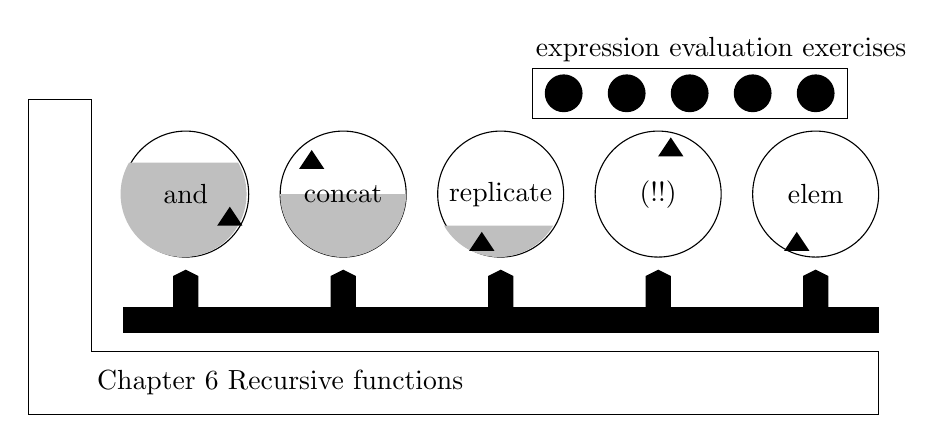
\begin{tikzpicture}[scale=0.08]

\foreach \x in {25,50,75,100,125}
     \draw (\x ,35) circle(10);
\node (sm) at (40,5) {Chapter 6 Recursive functions};
\fill[lightgray] (16,40) arc [start angle=150,   delta angle=240,
				x radius=10, y radius=10, color=lightgrey] -- cycle;
\node (o1) at (25,35) {and};
\fill[lightgray] (40,35) arc [start angle=180,   delta angle=180,
				x radius=10, y radius=10, color=lightgrey] -- cycle;
\node (o2) at (50,35) {concat};
\fill[lightgray] (66,30) arc [start angle=210,   delta angle=120,
				x radius=10, y radius=10, color=lightgrey] -- cycle;
\node (o3) at (75,35) {replicate};
\node (o4) at (100,35) {(!!)};
\node (o5) at (125,35) {elem};
\fill[black] (15,13) rectangle (135,17);
\foreach \x in {23,48,73,98, 123}
      \fill[black] (\x,17) -- (\x,22) -- (\x+2,23) -- (\x+4, 22) -- (\x+4,17) -- cycle;

\draw  (80,47) rectangle (130,55);
\foreach \x in {85,95,105, 115, 125}
\fill[black] (\x ,51) circle(3);
\node (eqr) at (110,58) {expression evaluation exercises}; 
\draw (0,0) -- (0,50) -- (10,50) -- (10,10) -- (135,10) -- (135,0) -- cycle;

\fill[black]  (30,30) -- (34,30) -- (32,33) -- cycle;
\fill[black]  (43,39) -- (47,39) -- (45,42) -- cycle;
\fill[black]  (70,26) -- (74,26) -- (72,29) -- cycle;
\fill[black]  (100,41) -- (104,41) -- (102,44) -- cycle;
\fill[black]  (120,26) -- (124,26) -- (122,29) -- cycle;


\end{tikzpicture}
\caption{Task class Recursive functions}\label{fig:taskclasserecursive}
\end{figure}




The four components in the \gls{tensteps} are depicted in figure \ref{fig:taskclasserecursive}.
Figure  \ref{fig:taskclasserecursive} is a possible task class modelled after chapter 6 ``Recusive functions'' of ``Programming in Haskell'' \citep{hutton_2016}.
The four components are the following:

\begin{itemize}
\item Learning tasks, grouped in task classes.\\
Each large circle in figure \ref{fig:taskclasserecursive} represents a learning task.
\item Supportive information.\\
The big L-shaped form represents supportive information. In this case the chapter from the textbook is used as supportive information.
The supportive material is made available in the beginning, probably supported with a lecture or a video. 
During the task class this is available at any moment.
\item Procedural information on routine aspects of the tasks.\\
The novice learner must be shown how to do it. 
A teacher may demonstrate the task execution, or give hints.
This, however, fades away during task class execution, as depicted by the grey areas in each circle.
\item Part-task practice to automate task aspects that are repeated often.\\
The small black circles depict part-task practice exercises for small aspects that must be carried out automatically.
\end{itemize}



\subsubsection{Learning tasks and task classes}
The major building blocks in the Ten Steps method are learning tasks, organized in task classes. 
Learning tasks must be authentic real-life whole-task learning experiences that integrate multiple skills, knowledge and attitudes.

The small triangles at different angles represent variability of the tasks. 
Variability is important for the development of schema-based processes in the mind.
Within a task class, the learning tasks must vary along the relevant dimensions.
For example, in the Lisp tutor it was discovered that students who had learned to define functions with one parameter started to
make errors when a function with two parameters was encountered \citep{corbett_1995}.
In that case the number of parameters is one dimension that must be varied.

Recursion comes in multiple forms.
Examples are recursive algorithms, mutual recursion, multiple recursion, tail recursion and recursion on lists.
The example of figure \ref{fig:taskclasserecursive} contains only exercises with recursion on lists.
The learner may get the impression that recursion is connected to  lists.

The tasks are grouped in task classes  of equal difficulty or complexity.
The task class is the unit of sequencing in Ten Steps. 
Task classes are usually of increasing complexity.  There is a prerequisite structure between task classes.
This does not necessarily imply a linear structure. 
It is possible to allow the learner to choose between options as long as prerequisites are met.

\subsubsection{Supportive information}
The learner receives supportive information when beginning a new task class. 
This can be a book, a presentation or even the Haskell language report.
The supportive information is presented in the beginning of the task class, and available during task execution.
The L-shaped form in \ref{fig:taskclasserecursive} represents supportive information.
This will explain the problems in the domain, solution strategies and mental models of how the domain is organised.


\subsubsection{Procedural information and procedural support}
\label{procsupport}
Procedural information supports the development of rule-based processes in the mind.
The tutor provides procedural information just in time as much as is needed.
In the beginning a demonstration may be given of the task, and later hints and feedback.
As the learner proceeds through the task class he will get more routine.
The procedural support then fades away.

The right amount of repetition is an important factor for rule-based processes.
When the learner can execute tasks without support he may proceed to a further task class.
It is not necessary that everyone completes all the tasks within the task class.
An \gls{its} needs a student model to provide this adaptivity.

\subsubsection{Part-task practice}

Learning tasks, as described above, are to practice real-life whole-tasks. 
Sometimes more practice is needed on a specific aspect of a complex skill.
In the domain of functional programming we may think of code reading and priority rules in expressions.
Applying parentheses rules and recognizing wrong or unnecessary use of parentheses is a valuable skill.
Part-task practice exercises offer an opportunity to drill these skills to be executed automatically.
In figure \ref{fig:taskclasserecursive} the part task practice is denoted by the small black circles in the right upper corner.



\subsection{Mapping the \gls{tensteps} to ITS design with domain reasoners.}

The \gls{tensteps} and \gls{its} world share similar concepts and methodologies, but use different terminology. 
An \gls{its} is one specific area where the \gls{tensteps} can be applied.

It is not required to execute all the steps. The four components are designed in ten steps.
Some artefacts are developed to support this design. 
These artefacts can also be used in the design of domain reasoners and student model.

A domain model is made, that contains important concepts and causal relations and structure of the knowledge domain.
This domain model can be used for both the student model and the design of supportive information.
It is useful if a Systematic Approach to Problem Solving (\gls{sap}) is available or can be constructed.
Such a \gls{sap} can be presented in supportive information and used to design strategies for domain reasoners.
Goals and prerequisites must be formulated for task classes and learning tasks, and assessment instruments developed.

In general \gls{its} design and the \gls{tensteps} use similar principles, but sometimes different terminology.
In the table \ref{map.tems} below we show how we apply the \gls{tensteps} to \gls{its} design.


\subsubsection{Learning tasks} 

\begin{table}[H]
\begin{tabular}{| p{5mm} |p{5cm}| p{8cm}|}
\hline
Step &Ten Steps concept & \gls{its} IDEAS concept \\
\hline
1 & Learning tasks      & Elements of the outer loop, \newline examples in IDEAS domain reasoner exercises     \\
2 & Assessment  & Diagnose service during exercise execution \\
3 & Sequence learning tasks & Outer loop \\
4 & Supportive information & Text books, references to documentation\\
5 & Cognitive Strategies & Rules and strategies in domain reasoners\\
5 & \gls{sap} & Design artefact for strategy and rule design\\
6 & Mental models & Used to structure our domain model: concepts, causal relations, structural relations\\
7 & Procedural support & Domain reasoner can generate a hint, next step, or a worked out solution\\
8 & Cognitive rules & Rules in domain reasoners, if then else rule, buggy rules\\
9 & Prerequisite knowledge & Must be checked automatically\\
10 & Part-Task practice & Small tasks to address an issue e.g. a missing prerequisite or misconception\\

\hline
\end{tabular}
\caption{Mapping of Ten Steps concepts}
\label{map.tems}
\end{table}







\section{PoSets and Lattices}
\label{sec:lattices}

In the next section we will show how lattices can be used in a student model.
This section presents a small review of lattice and poset terminology and properties.


\subsection{PoSets}

A partial ordering is a binary relation $ x \leq y$ in a set \citep{algebra}. 
A partial ordering has the following properties.
\begin{itemize}
\item Transitive, if $ a \leq b $ and $ b \leq c $ then $ a \leq c $.
\item Reflexive, the relation $\leq$ hold for any element with itself:  $ a \leq a $.
\item Anti-symmetric if $a \leq b $ and $ b \leq a$ then $ a  = b$.
\end{itemize}

A set with a partial ordering is called a poset.
If in a set this $\leq$ relation can be established for any two elements then we have a linear ordering.
In a partial ordering, there may be pairs of elements $(x,y)$ that are not comparable; neither $ x \leq y$ or $y \leq x$.
Some posets have an infimum denoted as $\bot$ or bottom,  or a supremum denoted as $\top$ or top.
In these case the following properties hold in the poset S:
\begin{itemize}
\item $ \forall x \in S: \bot \leq x $
\item $\forall x \in S: x \leq \top$
\end{itemize}


\subsection{Lattices}


Two elements $x$ and $y$ may not be comparable, but sometimes we can find elements that are greater or smaller.
If we can find an element $a$ such that $ a \leq x $ and $ a \leq y $, then $a$ is a lower bound of $x$ and $y$.
The binary operator meet ($\sqcup$) is defined as $ a = x \sqcup y $ where $a$ is the largest lower bound, 
there is no other element $a'$ such that $ a \leq a' $ and $ a' \leq x $ and $ a' \leq y $.

In a similar fashion we can define the operation join ($ \sqcap $): $ b = x \sqcap y$ if $ x \leq b $ and $ y \leq b $ and there is no other value $b'$ 
with $b' \leq b$ and  $ x \leq b' $ and $ y \leq b' $.

A poset with a meet and join operation is called a lattice.
A well known example of a lattice is the set with dividers of 60.
Meet is defined as the greatest common divisor e.g.: $12 \sqcup 10 = 2$, $20 \sqcup 15 = 5$.
Join is defined as the smallest common multiple e.g. $ 12 \sqcap 10 = 60$, $4 \sqcap 6 = 12$. 

\begin{Figure}
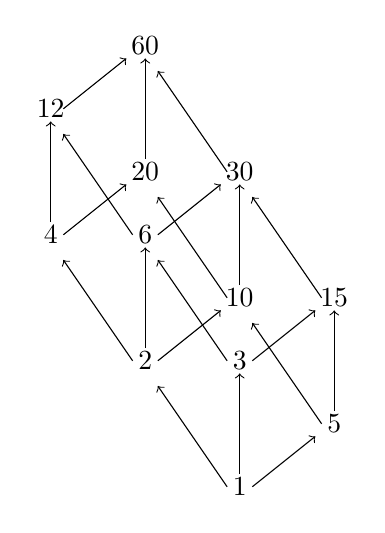
\begin{tikzpicture}[scale=0.08]

%\fill[black] (40,0) circle(1);
\node (o3) at (40,0) {1};
%\fill[black] (25,20) circle(1);
\node (o3) at (25,20) {2};
%\fill[black] (10,40) circle(1);
\node (o3) at (10,40) {4};

%\fill[black] (40,20) circle(1);
\node (o3) at (40,20) {3};
%\fill[black] (25,40) circle(1);
\node (o3) at (25,40) {6};
%\fill[black] (10,60) circle(1);
\node (o3) at (10,60) {12};

%\fill[black] (55,10) circle(1);
\node (o3) at (55,10) {5};
%\fill[black] (40,30) circle(1);
\node (o3) at (40,30) {10};
%\fill[black] (25,50) circle(1);
\node (o3) at (25,50) {20};

%\fill[black] (55,30) circle(1);
\node (o3) at (55,30) {15};
%\fill[black] (40,50) circle(1);
\node (o3) at (40,50) {30};
%\fill[black] (25,70) circle(1);
\node (o3) at (25,70) {60};



\draw [->] (40,2) -- (40,18);   %1-3
\draw [->] (55,12) -- (55,28); % 5-15
\draw [->] (25,22) -- (25,38);
\draw [->] (40,32) -- (40,48);
\draw [->] (25,52) -- (25,68);
\draw [->] (10,42) -- (10,58);

\draw [->] (42,0) -- (52,8);     % 1- 5
\draw [->] (42,20) -- (52,28);
\draw [->] (27,20) -- (37,28);
\draw [->] (27,40) -- (37,48);
\draw [->] (12,40) -- (22,48);
\draw [->] (12,60) -- (22,68);

\draw [->] (38,0) -- (27,16);  % 1-2
\draw [->] (23,20) -- (12,36);
\draw [->] (53,10) -- (42,26);
\draw [->] (38,30) -- (27,46);

\draw [->] (38,20) -- (27,36); 
\draw [->] (23,40) -- (12,56);
\draw [->] (53,30) -- (42,46);
\draw [->] (38,50) -- (27,66);


\end{tikzpicture}
\caption{Hasse diagram for dividers of 60}\label{fig:hasse}
\end{Figure}

Figure \ref{fig:hasse} shows a Hasse diagram for this system of dividers of 60. 
This diagram is based on the concept of immediate successor and predecessor.
In this diagram 10 is an immediate predecessor of 30, written as $ 10 \ll 30$ since there
is no element greater than 10 preceding 30. 
We cannot say $ 10 \leq 15$, in this algebra there is no linear ordering and the numbers are not comparable.
In a finite lattice there is always a bottom and a top, in this case 1 and 60.

Boolean values form a lattice. 
A finite or infinite interval of integer numbers forms a lattice when join is chosen as max and meet as min.
Similar any ordered enumeration forms a lattice. 

An important property is that lattices can be combined. 
If A and B are lattices then tuples $(a, b) \in  A \times B$ form a lattice.

Equations \ref{eq:ABmeet} through \ref{eq:bottomtupe} show how meet, join, less or equal and bottom for $A \times B$ can be defined.
\begin{equation}
\label{eq:ABmeet}
(a_{1}, b_{1}) \sqcap (a_{2}, b_{2})  = ( a_{1} \sqcap a_{2}, b_{1} \sqcap b_{2}) 
\end {equation}
\begin{equation}
(a_{1}, b_{1}) \sqcup (a_{2}, b_{2})  = ( a_{1} \sqcup a_{2}, b_{1} \sqcup b_{2}) 
\end {equation}
\begin{equation}
(a_{1}, b_{1}) \leq (a_{2}, b_{2})  =  a_{1} \leq a_{2} \land   b_{1} \leq b_{2} 
\end {equation}
\begin{equation}
\label{eq:bottomtupe}
\bot_{A \times B}  =  (\bot_{A}, \bot_{B})
\end {equation}
 
This can be extended to any number of dimensions. 
If C is a lattice, then in a similar way the set $(a, b, c) \in A \times B \times C$ forms a three dimensional lattice.


\subsubsection{Duality} 
Lattices have a duality property.
We can exchange the $\sqcup$ and $\sqcap$, the $\leq$ and $\geq$ and in finite lattices $\bot$ and $\top$.
The result is a new lattice.
In a similar fashion alternative definition can be made for equations \ref{eq:ABmeet} through \ref{eq:bottomtupe}.
To avoid confusion we will not do this.




















